\subsection{Разряды}

Шестнадцатиразрядные регистры DS ,ES, FS, GS, четыре сегментных регистра используются для определения начала сегментов данных.

CS "--- сегментный регистр сегмента кода, SS "--- сегмента стека.
Операционные системы могут размещать сегменты в ОП произвольным образом и даже временно записывать их на диск, если есть
нехватка оперативной памяти. Эти сегменты называются селекторами, они доступны программисту. 

С каждого сегмента есть программно-недоступный регистр называемый дескриптором. И в защищенном режиме именно в дескрипторе находится адрес
начала сегмента, его размер и некоторые другие аттрибуты. 

В реальном режиме, который чаще всего используется, размер
сегмента фиксирован, равен 64 Кбайтам, адрес сегмента кратен 16, поэтому в Шестнадцатиричной системе он записан
как 4 Шестнадцатиричные цифры и 0 (XXXX0).

В защищенном режиме размер может достигать до 4 Гбайт.

Всего сегментных регистров шесть, однако программист может в любой момент изменить содержимое сегментного регистра, таким
образом попасть в другой участок оперативной памяти. Например, если изменить содержимое регистра CS, процессор попадет
на выполнение другой программы "--- программы, содержащейся в другом участке памяти. Это может быть подпрограмма, либо
системно"=обрабатывающая программа.

Особенным образом реализуется SS. Адрес начала SS операционная система автоматически записывает в регистр SS. А указателем
на вершину стека является регистр SP "--- Stack Pointer, причем при добавлении элемента в стек содержимое регистра SP уменьшается.
Иными словами, стек растёт от максимально возможного значения вниз.

Такая реализация оказывается необходимой при работе с памятью в режиме flat, когда программа размещается в младших адресах
и с увеличением команды адреса растут, а стек размещается в старших адресах.

Если в стеке мы хотим хранить и фактические параметры, и локальные, то после загрузки фактических параметров в стек
указатель на вершину стека можно сохранять в специальном регистре Base Pointer(BP), И продолжая размещать локальные
параметры в стеке, мы сможем обращаться к фактическим параметрам, используя выражение $BP + k$, а к локальным $BP - r$,
где $k$ и $n$ "--- определяются количеством параметров и их размером.

Регистр flags определяет состояние программ и процессора в каждый текущий момент времени. Это 32-разрядный регистр, 
в котором 1, 3, 5, 15, 19-31 биты не используются. Девять флагов используются и в реальном, и в защищенном режиме,
следующие пять "--- только в защищенном режиме. Из девяти первых флагов шесть определяют состояние программы, а три определяют
состояние работы процессора. 

\begin{figure}[H]
    \centering
    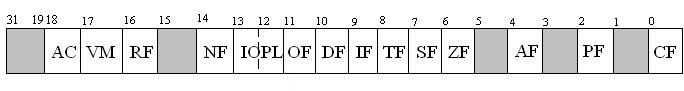
\includegraphics[scale = 0.5]{flags.jpg}
\end{figure}


\begin{enumerate}
\item CF "--- флаг переноса. Устанавливается в единицу, если при сложении происходит перенос за разрядную сетку, а при вычитании
требуется заём. 
\item FF "--- флаг четности. Устанавливается в единицу, если в младшем байте результата окажется четное количество единиц.
\item AF "--- флаг полупереноса. Устанавливается в единицу, если при сложении(вычитании) происходит перенос из третьего разряда
в четвертый(требуется заём из четвертого в третий)
\item ZF "--- флаг нуля. Устанавливается в единицу, если все разряды результата равны нулю.
\item SF "--- флаг знака. Всегда равен знаковому разряду результата. Положительный результат "--- ноль, отрицательный "--- единица.
\item TF "--- флаг трассировки. Установленный в единицу переводит процессор в режим пошагового выполнения программы.
\item IF "--- флаг прерывания. Установленный в единицу, позволяет остановить обработку некоторых прерываний.
\item DF "--- флаг направления. Определяет режим работы со строками. Если DF равен нулю, строка обрабатывается в сторону старших
адресов, в сторону младших в противном случае. При этом автоматически увеличивается(уменьшается) содержимое индексных регистров
если DF = 0 (DF = 1).
\item OF "--- флаг переполнения. Устанавливается в единицу, если результат превышает максимально допустимый для данной разрядной
сетки.
\item AC "--- флаг выравнивания операндов. Установленный в единицу, вызовет сообщение об ошибке, если адреса слов и двойных слов
не кратны двум или четырем соответственно.
\item VM "--- флаг виртуальных машин. Установленный в единицу, ползволяет перевести процессор в режим виртуальных машин.
\item RF "--- флаг маскирования прерывания. Позволяыет запретить прерывание.
\item NT "--- флаг вложенной задачи. Позволяет перейти в режим вложенной задачи.
\item IOPL "--- флаг уровня привелегий текущей программы. Если он окажется меньше значения флага, то программе будут запрещены
операции ввода/вывода.
\end{enumerate} 

\subsection{Оперативная память (RAM)}

Оперативная память состоит из байтов. Байт состоит из восьми информационных битов. Разряды с нулевого по третий "---
цифровая часть байта, с четвертого по седьмой "--- зонная часть байта.
\begin{figure}[H]
    \centering
    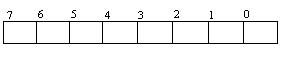
\includegraphics[scale = 0.5]{ram.jpg}
\end{figure}
32-х разрядный процессор может работать с оперативной памятью до 4 Гб, а значит физический адрес байта может изменяться от 
0 до $2^32 - 1$, что в Шестнадцатиричной системе записывается как $00000000 -> FFFFFFFF$.

Байты могут объединяться в поля фиксированной и переменной длины. Такие поля имеют собственные имена "--- слово (2 байта), двойное слово (4 байта).
Поле переменной длины может состоять из произвольного количества байтов. Адресом такого поля может быть адрес любого байта,
но это адрес младшего байта, входящего в поле.

Поле может использоваться как непрерывная память, либо сегментированная. В случае, если память сегментирована, то память
записывается как <сегмент>: <смещение>, а вычислено может быть по формуле ФА = АС + ИА, где АС - опредяется сегметным регистром,
а ИА "--- смещение сегмента, формируемое в команде и зависит от способа адрессации операнда.

В защищенном режиме программа может определять до 16383 сегментов размером до 4 Гб, и таким образом работать с 
64 ТБайтами виртуальной памяти.

Для реального режима адрес сегмента определяется сегментным регистром, и для получения 20-разрядного двоичного адреса
байта содержимое сегментного регистра, смещенного на 4 разряда влево прибавляют смещение (ИА).

\section{Работа с ассемблером}
\subsection{Форматы данных}

Процессор ix86 вместе с сопроцессором могут обрабатывать целые числа без знака, целые числа со знаком, действительные с плавающей
точкой, двоично-десятичные, символы, строки, указатели.
\paragraph{Целые числа.}

Целые двоичные без знака могут занимать байт, слово или двойное слово и принимать числа из диапазона 0-255, 0-65535, 0-4294967295
соответственно.
Целые числа со знаком так же могут занимать байт, слово или двойное слово, но представляются в дополнительном коде.

Дополнительнй код положительного числа совпадает с записью числа, а дополнительный код отрицательного числа может быть получен по
формуле $X = 10^n - |X|$.
Дополнительный код двоичного числа можно получить инверсией всех разрядов числа и добавление единицы к младшему разряду.

Вычитание в машине заменяется сложением уменьшаемого и доп. кодом вычитаемого числа. 
Действительные числа(числа с плавающей точкой) могут занимать 32 разряда (короткое), 64 разряда (длинное), 80 разрядов (рабочее).
Формат числа с плавающей точкой состоит из трех полей: знак числа, машинный порядок и мантисса.

Порядки:

$1 + 8 + 23 -> -10^{+-32} - 10^{+-32}$

$1 + 11 + 52$

$1 + 15+ 64$

Машинный порядок неявным образом включает в себя знак порядка. Он связан истинным следующим соотношением: $P_m = P_i + 127(1023, 16383)$.
Мантисса должна быть нормализованной, и старшая единица в разрядную сетку не помещается для экономии памяти.

\paragraph{Двоично"=десятичные числа.}

Процессор может обратаывать двоично"=десятичные числа в упакованном или неупакованном формате, а 
сопроцессором могут обрабатываться 90-ти разрядные данные в упакованном формате.

Они неупакованные "--- одну цифру в одной части байта.

\paragraph{Символы.}

Для символом используется кодировка ASCII. Для любого символа отводится один байт.
Строковые данные являются последовательностью байтов, слов или двойных слов.

Указатели на строку подразделяются на два типа:
длинный указатель, занимающий 48 бит (32 смещение + 16 сегмент)
короткий указатель, занимающий 32 бита(32 смещение)

\subsection{Форматы команд}

Команды "--- последовательность нулей или единиц, состоящих из двух подпоследовательностей.
Одна из них определяет код операции (сложить, умножить и т.~д), а другая определяет адреса операндов
и адрес размещения результата команды.

Операндами могут быть байтом, словом или двойным словом. Команда в свою очередь может быть безадресной, 
одноадресной, двухадресной или трехадресной.

В памяти команда может занимать от одного до 15 байтов, в зависимости от кода операции, количества и
размера операндов. Операнды могут находиться в команде, в регистрах или памяти. В одноадресной команде
операнд находится или в регистре, или в памяти, самое большое количество команд "--- двухадресные.

Существуют различные форматы двухадресных команд, которые отличаются расположением команд.
Регистр"=регистр, память"=память, регистр"=память, память"=регистр, данные"=память, память"=данные.

В общем случае, исполняемый адрес может состоять из трех частей: база, индекс и смещение.
Существуют различные способы способы адресации операндов, такие как:
\begin{enumerate}
    \item регистровая
    \item непосредственная
    \item прямая
    \item косвенно"=регистровая
    \item по базе со смещением
    \item прямая с индексированием
    \item по базе с индексированием (двумерные массивы)
    \item косвенная адресация с масштабированием
    \item базово"=индексная с масштабированием
    \item базово"=индексная с масштабированием и смещением
    
\end{enumerate}

